\begin{frame}

\begin{minipage}{0.4\textwidth}
    Some bullshit
\end{minipage}
\begin{minipage}{0.5\textwidth}
% \begin{tikzpicture}
%     \node[anchor=south west,inner sep=0] (image) at (0,0) {
%         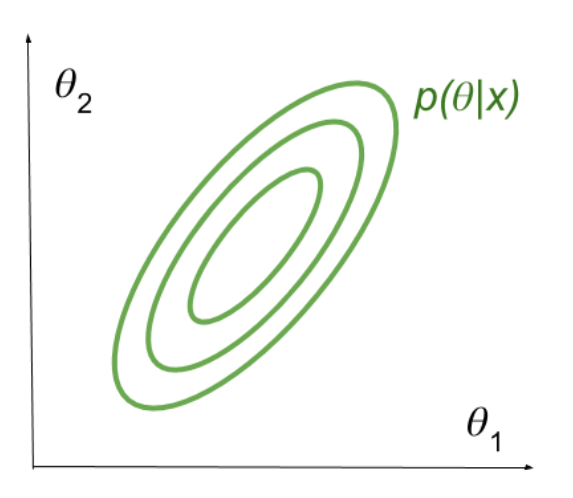
\includegraphics[width=1.0\textwidth]{static_images/bvn_target.png}
%     };
%     \begin{scope}[x={(image.south east)},y={(image.north west)}]
%         \draw[black, thick, fill=white]
%             (0.46,0.2) -- ++(0.2,0) -- ++(0,0.65) -- ++(-0.2,0) -- cycle;
%     \end{scope}
% \end{tikzpicture}


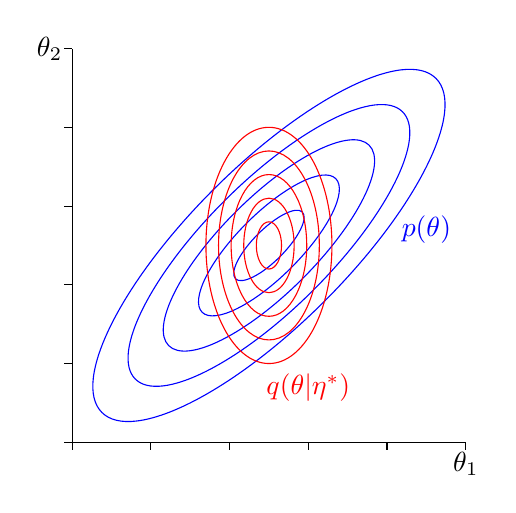
\begin{tikzpicture}
 \draw (0,0)--(5,0);
\foreach \x in {0,...,5}
  \draw (\x,0)--(\x,-.1) node[anchor=north]{};

\draw (0,0)--(0,5);
\foreach \y in {0,...,5}
  \draw (0,\y)--(-.1,\y) node[anchor=east] {};

\draw (0,5) node[anchor=east] {$\theta_2$};
\draw (5,0) node[anchor=north] {$\theta_1$};

\draw[blue] (4.5, 3)  node[anchor=north] {$p(\theta)$};
\begin{scope}[shift={(2.5,2.5)}]
    \begin{scope}[rotate=45]
        \begin{scope}[shift={(-2.5,-2.5)}]
            \foreach \s in {0.2, 0.4, 0.6, 0.8, 1.0}
            \draw[blue] (2.5,2.5) ellipse (\s * 3 and \s * 1);
        \end{scope}
    \end{scope}
\end{scope}


\draw[red] (3, 1)  node[anchor=north] {$q(\theta | \eta^*)$};
\foreach \s in {0.2, 0.4, 0.6, 0.8, 1.0}
    \draw[red] (2.5,2.5) ellipse (\s * 0.8 and \s * 1.5);


\end{tikzpicture}
\end{minipage}

\end{frame}
